\chapter{Project Requirements [AS PER FYP1 MID REPORT]}
This chapter describes the functional and non-functional requirements of the project. 
\section{Use-cases}
The Table 2.1 lists down all the possible use cases for our project. 
Note that login, sign up and feedback pages are not included in these use cases.
% ---------- Summary Table ----------
\begin{table}[htbp]
\caption{Summary of Use Cases for ForeSyte}
\centering
\begin{tabular}{|c|p{4cm}|p{8cm}|}
\hline
\textbf{Usecase ID} & \textbf{Use Case Name} & \textbf{Description} \\ \hline
UC-01 & View \& Manage Reports/Dashboard & Authorized users view and manage reports of student and invigilator activity. \\ \hline
UC-02 & Manage User Profiles & System administrator manages accounts and roles of all users. \\ \hline
UC-03 & Generate Detection Reports & System generates timestamped reports of detected cheating or negligence. \\ \hline
UC-04 & Verify Student Identity \& Seat Mapping & System verifies student identity using face recognition and assigned seats. \\ \hline
UC-05 & Monitor Invigilator Activity & System monitors invigilators for negligence, absence, or unauthorized actions. \\ \hline
UC-06 & Monitor Student Behaviour & System monitors student actions to detect cheating attempts. \\ \hline
UC-07 & Process Exam Footage (Live/Recorded) & System processes live and recorded video streams to detect activities. \\ \hline
\end{tabular}
\end{table}
\vspace{0.5cm} % <-- add some vertical space

% Text outside tables
  Below, you can find the detailed use case description for each use case.
\clearpage

% ---------- UC-01 ----------
\subsubsection*{2.1.1\quad UC-01}

\begin{longtable}{|p{5cm}|p{10cm}|}
\caption{Use Case 1: View \& Manage Reports/Dashboard} \label{uc1} \\

\hline
\textbf{Use Case Detail} & \textbf{Description} \\ \hline
Use Case ID & UC-01 \\ \hline
Use Case Name & View \& Manage Reports/Dashboard \\ \hline
Scope & ForeSyte Web Portal \\ \hline
Level & User Goal \\ \hline
Brief Description & Users view, filter, and manage real-time dashboards and past reports. \\ \hline
Actor(s) Involved & System Administrator, Investigator, Discipline Committee \\ \hline
Stakeholders & • Discipline Committee: Reviews violation data \newline • Admins: Configure reports \\ \hline
Pre-conditions & Reports and logs already generated by detection system. \\ \hline
Post-conditions & Users access detailed dashboards with downloadable reports. \\ \hline
Main Success Scenario & 
1. Actor logs into the ForeSyte Web Portal successfully. \newline
2. Actor navigates to the Reports/Dashboard section from the main menu. \newline
3. System retrieves all available violation reports from the database. \newline
4. System displays a dashboard with filters (e.g., by student ID, seat number, violation type, or timestamp). \newline
5. Actor applies filters to refine the report view. \newline
6. System dynamically updates the dashboard according to the selected filters. \newline
7. Actor selects a specific report for detailed view. \newline
8. System displays complete details of the selected report (student, invigilator, time, violation evidence). \newline
9. Actor chooses the option to download or export the report. \newline
10. System generates the report in the selected format (PDF/Excel) and confirms successful export. \\ \hline

Special Requirements & Role-based access, secure data visualization \\ \hline

\end{longtable}

\clearpage

% ---------- UC-02 ----------
\subsubsection*{2.1.2\quad UC-02}
\begin{longtable}{|p{5cm}|p{10cm}|}
\caption{Use Case 2: Manage User Profiles} \label{uc1} \\
\hline

\textbf{Use Case Detail} & \textbf{Description} \\ \hline
Use Case ID & UC-02 \\ \hline
Use Case Name & Manage User Profiles \\ \hline
Scope & ForeSyte Web Portal \\ \hline
Level & User Goal \\ \hline
Brief Description & System administrator manages user accounts, roles, and permissions. \\ \hline
Actor(s) Involved & System Administrator \\ \hline
Stakeholders & • Admins: Maintain structured access \\ \hline
Pre-conditions & Admin is authenticated. \\ \hline
Post-conditions & User accounts created, modified, or deleted. \\ \hline
Main Success Scenario & 
1. Admin logs into the ForeSyte Web Portal. \newline
2. Admin navigates to the User Management module. \newline
3. System displays the list of existing users with their roles. \newline
4. Admin selects an action (add, edit, or delete a user). \newline
5. If adding: Admin enters new user details including username, role, and credentials. \newline
6. If editing: Admin updates user details or permissions. \newline
7. If deleting: Admin selects a user and confirms deletion. \newline
8. System validates the request and updates the database accordingly. \newline
9. System confirms success with a message (user added/updated/deleted). \newline
10. Admin logs out or continues with further management tasks. \\ \hline

Special Requirements & Secure password policies, role-based restrictions \\ \hline

\end{longtable}

\clearpage

% ---------- UC-03 ----------
\subsubsection*{2.1.3\quad UC-03}
\begin{longtable}{|p{5cm}|p{10cm}|}
\caption{Use Case 3: Generate Detection Reports}\label{uc1} \\
\hline
\textbf{Use Case Detail} & \textbf{Description} \\ \hline
Use Case ID & UC-03 \\ \hline
Use Case Name & Generate Detection Reports \\ \hline
Scope & Backend Service + Web Portal \\ \hline
Level & User Goal \\ \hline
Brief Description & System generates timestamped detection reports of suspicious activity. \\ \hline
Actor(s) Involved & Investigator, Discipline Committee \\ \hline
Stakeholders & • Discipline Committee: Reviews reports \newline • University Management \\ \hline
Pre-conditions & Detection system has analyzed video footage. \\ \hline
Post-conditions & Report generated and stored in database. \\ \hline
Main Success Scenario & 
1. AI detection engine processes exam footage. \newline
2. System identifies suspicious activity (e.g., phone usage, looking around, invigilator negligence). \newline
3. System logs details including timestamp, seat number, room, and involved actor. \newline
4. System compiles the violation data into a structured report format. \newline
5. Investigator accesses the Web Portal and navigates to the Reports section. \newline
6. System displays the list of generated reports. \newline
7. Investigator selects a specific report for review. \newline
8. System displays detailed evidence including video snippets or screenshots. \newline
9. Investigator verifies and approves the report for further review. \newline
10. Report is stored in the system and available for export (PDF/Excel). \\ \hline

Special Requirements & Reports exportable to PDF/Excel \\ \hline

\end{longtable}

\clearpage

% ---------- UC-04 ----------
\subsubsection*{2.1.4\quad UC-04}
\begin{longtable}{|p{5cm}|p{10cm}|}
\caption{Use Case 4: Verify Student Identity \& Seat Mapping}\label{uc1} \\
\hline
\textbf{Use Case Detail} & \textbf{Description} \\ \hline
Use Case ID & UC-04 \\ \hline
Use Case Name & Verify Student Identity \& Seat Mapping \\ \hline
Scope & Backend Service \\ \hline
Level & User Goal \\ \hline
Brief Description & System verifies student identity using face recognition and seat mapping. \\ \hline
Actor(s) Involved & Student, Invigilator \\ \hline
Stakeholders & • University Management \\ \hline
Pre-conditions & Seating plan and student ID data available. \\ \hline
Post-conditions & Student identity verified and mapped. \\ \hline
Main Success Scenario & 
1. Exam seating plan is uploaded into the system. \newline
2. Student enters the exam hall and sits on the assigned seat. \newline
3. System activates facial recognition through CCTV or camera feed. \newline
4. System captures the student’s face and compares it with pre-stored student records. \newline
5. System checks whether the student is seated in the correct assigned seat. \newline
6. If the identity matches, the system confirms successful verification. \newline
7. If there is a mismatch, the system flags the seat for manual review by the examiner. \newline
8. System logs the verification results along with seat ID and student ID. \newline
9. Verified data is linked to subsequent activity monitoring and reports. \\ \hline
Special Requirements & Reliable face recognition with low error rate \\ \hline


\end{longtable}

\clearpage

% ---------- UC-05 ----------
\subsubsection*{2.1.5\quad UC-05}
\begin{longtable}{|p{5cm}|p{10cm}|}
\caption{Use Case 5: Monitor Invigilator Activity}\label{uc1} \\
\hline
\textbf{Use Case Detail} & \textbf{Description} \\ \hline
Use Case ID & UC-05 \\ \hline
Use Case Name & Monitor Invigilator Activity \\ \hline
Scope & Backend Service \\ \hline
Level & User Goal \\ \hline
Brief Description & System tracks invigilators for negligence, absence, or unauthorized actions. \\ \hline
Actor(s) Involved & Invigilator, Discipline Committee \\ \hline
Stakeholders & • University Management \\ \hline
Pre-conditions & Cameras active and invigilator zones defined. \\ \hline
Post-conditions & Invigilator activity log generated. \\ \hline
Main Success Scenario & 
1. Surveillance cameras start recording invigilator activity. \newline
2. System tracks invigilator’s presence across different zones of the exam hall. \newline
3. AI analyzes the video feed to detect movement or prolonged inactivity. \newline
4. If invigilator leaves their zone for too long, the system flags negligence. \newline
5. If invigilator is using unauthorized devices (e.g., phone), system captures it. \newline
6. System logs the timestamp, location, and detected action. \newline
7. Discipline Committee accesses the dashboard to view invigilator logs. \newline
8. System displays flagged negligence cases in the report. \newline
9. Committee reviews and validates the report. \newline
10. Finalized invigilator activity log is stored and exported if needed. \\ \hline

Special Requirements & Accurate zone mapping \\ \hline

\end{longtable}

\clearpage

% ---------- UC-06 ----------
\subsubsection*{2.1.6\quad UC-06}
\begin{longtable}{|p{5cm}|p{10cm}|}
\caption{Use Case 6: Monitor Student Behaviour}\label{uc1} \\
\hline
\textbf{Use Case Detail} & \textbf{Description} \\ \hline
Use Case ID & UC-06 \\ \hline
Use Case Name & Monitor Student Behaviour \\ \hline
Scope & Backend Service \\ \hline
Level & User Goal \\ \hline
Brief Description & Detects cheating behaviors (phone use, gestures, looking around). \\ \hline
Actor(s) Involved & Student, Investigator \\ \hline
Stakeholders & • Discipline Committee \newline • University Management \\ \hline
Pre-conditions & Camera feed and detection models active. \\ \hline
Post-conditions & Violations logged with timestamps. \\ \hline
Main Success Scenario & 
1. Exam begins and surveillance cameras monitor all students. \newline
2. AI detection model continuously analyzes student actions. \newline
3. System identifies suspicious behavior such as phone use, hand gestures, or looking around repeatedly. \newline
4. When detected, system flags the behavior as a potential violation. \newline
5. System records timestamp, seat ID, and video evidence. \newline
6. Investigator accesses the dashboard to review logged violations. \newline
7. System displays detailed violation logs with associated video frames. \newline
8. Investigator examines the evidence for each flagged action. \newline
9. Investigator confirms or dismisses the violation. \newline
10. Validated violations are added to the final exam report. \\ \hline
Special Requirements & Must differentiate normal vs cheating actions \\ \hline

\end{longtable}

\clearpage

% ---------- UC-07 ----------
\subsubsection*{2.1.7\quad UC-07}
\begin{longtable}{|p{5cm}|p{10cm}|}
\caption{Use Case 7: Process Exam Footage (Live/Recorded)}\label{uc1} \\
\hline
\textbf{Use Case Detail} & \textbf{Description} \\ \hline
Use Case ID & UC-07 \\ \hline
Use Case Name & Process Exam Footage (Live/Recorded) \\ \hline
Scope & Backend Service \\ \hline
Level & User Goal \\ \hline
Brief Description & System processes live and recorded exam video footage for analysis. \\ \hline
Actor(s) Involved & System Administrator, Investigator \\ \hline
Stakeholders & • University Management \\ \hline
Pre-conditions & Camera streams or uploaded recordings available. \\ \hline
Post-conditions & Footage analyzed and results stored. \\ \hline
Main Success Scenario & 
1. System connects to live CCTV cameras or receives uploaded exam recordings. \newline
2. System validates video input and prepares it for analysis. \newline
3. AI engine processes video frames in real time or batch mode. \newline
4. System identifies and logs suspicious student or invigilator behavior. \newline
5. System maps detected activity to the correct student seat. \newline
6. All activities are logged with timestamps and stored in the database. \newline
7. Investigator accesses the Reports module. \newline
8. System displays results of processed footage (violations, seat mapping). \newline
9. Investigator reviews the logged activities and evidence. \newline
10. Reports are finalized and exported in required format. \\ \hline

Special Requirements & Efficient processing, storage optimization \\ \hline

\end{longtable}
\clearpage
% ---------- Use Case Diagram ----------
\subsection*{2.1.8\quad Use Case Diagram of ForeSyte}

The Figure \textcolor{blue}{\ref{fig:usecase}} highlights the use case diagram of the entire ForeSyte Web Application.


\begin{figure}[htbp]
    \centering
    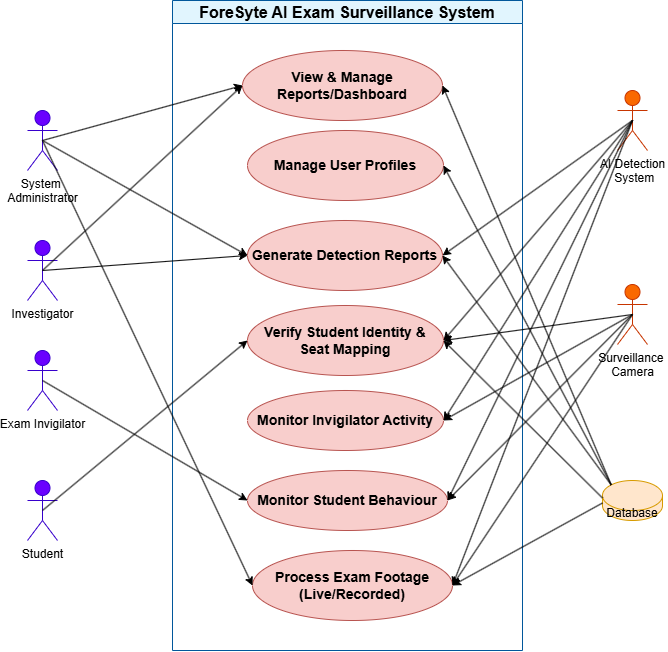
\includegraphics[width=\textwidth]{sections/usecase.png}
    \caption{ForeSyte Use Case Diagram}
    \label{fig:usecase}
\end{figure}

\section{Functional Requirements}
This section describes the functional requirements of ForeSyte arranged in a use case-based organizational method.

% ---------- UC-01 ----------
\subsubsection*{2.2.1\quad UC-01 Functional Requirement}
\vspace{-0.5em}
\begin{table}[H]
\caption{Functional Requirements for UC-01}
\centering
\begin{tabular}{|c|p{11cm}|}
\hline
\textbf{Functional Requirement ID} & \textbf{Description} \\ \hline
FR-01 & The system shall allow authorized users to log in and access the Reports/Dashboard module. \\ \hline
FR-02 & The system shall display real-time and historical reports of student and invigilator activity. \\ \hline
FR-03 & The system shall provide filtering options (by student ID, seat number, violation type, timestamp). \\ \hline
FR-04 & The system shall allow exporting reports in PDF and Excel formats. \\ \hline
FR-05 & The system shall enforce role-based access to reports. \\ \hline
\end{tabular}
\end{table}

% ---------- UC-02 ----------
\subsubsection*{2.2.2\quad UC-02 Functional Requirement}
\vspace{-0.5em}
\begin{table}[H]
\caption{Functional Requirements for UC-02}
\centering
\begin{tabular}{|c|p{11cm}|}
\hline
\textbf{Functional Requirement ID} & \textbf{Description} \\ \hline
FR-06 & The system shall allow the administrator to add new user accounts with role assignments. \\ \hline
FR-07 & The system shall allow editing of existing user details and permissions. \\ \hline
FR-08 & The system shall allow deleting user accounts securely. \\ \hline
FR-09 & The system shall validate inputs (username, password, role) before saving. \\ \hline
FR-10 & The system shall enforce strong password and security policies. \\ \hline
\end{tabular}
\end{table}

% ---------- UC-03 ----------
\subsubsection*{2.2.3\quad UC-03 Functional Requirement}
\vspace{-0.5em}
\begin{table}[H]
\caption{Functional Requirements for UC-03}
\centering
\begin{tabular}{|c|p{11cm}|}
\hline
\textbf{Functional Requirement ID} & \textbf{Description} \\ \hline
FR-11 & The system shall automatically generate detection reports when violations are flagged. \\ \hline
FR-12 & The system shall include timestamps, seat numbers, and violation type in reports. \\ \hline
FR-13 & The system shall store generated reports in a database. \\ \hline
FR-14 & The system shall allow investigators to review and approve reports. \\ \hline
FR-15 & The system shall allow reports to be exported in PDF/Excel format. \\ \hline
\end{tabular}
\end{table}

% ---------- UC-04 ----------
\subsubsection*{2.2.4\quad UC-04 Functional Requirement}
\vspace{-0.5em}
\begin{table}[H]
\caption{Functional Requirements for UC-04}
\centering
\begin{tabular}{|c|p{11cm}|}
\hline
\textbf{Functional Requirement ID} & \textbf{Description} \\ \hline
FR-16 & The system shall verify student identity using face recognition. \\ \hline
FR-17 & The system shall cross-check student identity against pre-stored records. \\ \hline
FR-18 & The system shall map verified students to their assigned seat numbers. \\ \hline
FR-19 & The system shall log verification results (student ID, seat ID, verification status). \\ \hline
FR-20 & The system shall flag mismatches for manual review. \\ \hline
\end{tabular}
\end{table}

% ---------- UC-05 ----------
\subsubsection*{2.2.5\quad UC-05 Functional Requirement}
\vspace{-0.5em}
\begin{table}[H]
\caption{Functional Requirements for UC-05}
\centering
\begin{tabular}{|c|p{11cm}|}
\hline
\textbf{Functional Requirement ID} & \textbf{Description} \\ \hline
FR-21 & The system shall monitor invigilators during exam sessions. \\ \hline
FR-22 & The system shall track invigilator presence in defined zones. \\ \hline
FR-23 & The system shall detect unauthorized activities (e.g., phone use). \\ \hline
FR-24 & The system shall log negligence events with timestamp and location. \\ \hline
FR-25 & The system shall provide invigilator activity logs to the Discipline Committee. \\ \hline
\end{tabular}
\end{table}

% ---------- UC-06 ----------
\subsubsection*{2.2.6\quad UC-06 Functional Requirement}
\vspace{-0.5em}
\begin{table}[H]
\caption{Functional Requirements for UC-06}
\centering
\begin{tabular}{|c|p{11cm}|}
\hline
\textbf{Functional Requirement ID} & \textbf{Description} \\ \hline
FR-26 & The system shall analyze student actions in real time. \\ \hline
FR-27 & The system shall detect suspicious behaviors (phone use, hand gestures, looking around). \\ \hline
FR-28 & The system shall differentiate between normal and abnormal behaviors. \\ \hline
FR-29 & The system shall log violations with seat ID, timestamp, and video snippet. \\ \hline
FR-30 & The system shall allow investigators to review and confirm logged violations. \\ \hline
\end{tabular}
\end{table}

% ---------- UC-07 ----------
\subsubsection*{2.2.7\quad UC-07 Functional Requirement}
\vspace{-0.5em}
\begin{table}[H]
\caption{Functional Requirements for UC-07}
\centering
\begin{tabular}{|c|p{11cm}|}
\hline
\textbf{Functional Requirement ID} & \textbf{Description} \\ \hline
FR-31 & The system shall process both live CCTV feeds and uploaded recordings. \\ \hline
FR-32 & The system shall analyze frames using AI detection models. \\ \hline
FR-33 & The system shall log activities with timestamps and seat IDs. \\ \hline
FR-34 & The system shall store processed results in the database. \\ \hline
FR-35 & The system shall make analyzed results available in the Reports module. \\ \hline
\end{tabular}
\end{table}

% ---------- General ----------
\subsubsection*{2.2.8\quad General Functional Requirements}
\vspace{-0.5em}
\begin{table}[H]
\caption{General Functional Requirements}
\centering
\begin{tabular}{|c|p{11cm}|}
\hline
\textbf{Functional Requirement ID} & \textbf{Description} \\ \hline
FR-36 & The system shall ensure processing of violations and reports within 20 seconds. \\ \hline
FR-37 & The system shall implement secure storage and encryption of student/exam data. \\ \hline
FR-38 & The system shall allow a responsive web interface for investigators and administrators. \\ \hline
FR-39 & The system shall maintain audit logs for all activities. \\ \hline
FR-40 & The system shall support scalability for multiple exam halls simultaneously. \\ \hline
\end{tabular}
\end{table}
\subsection*{2.2.9\quad Module 1: ForeSyte Web Portal}
Following are the requirements for Module 1 (ForeSyte Web Portal):

\begin{enumerate}
    \item \textbf{Dashboard Visualization}
    \begin{enumerate}[label=(\alph*)]
        \item FR-01: The system shall allow authorized users to log in and access the Reports/Dashboard module.
        \item FR-02: The system shall display real-time and historical reports of student and invigilator activity.
        \item FR-03: The system shall provide filtering options (by student ID, seat number, violation type, timestamp).
        \item FR-04: The system shall allow exporting reports in PDF and Excel formats.
        \item FR-05: The system shall enforce role-based access to reports.
    \end{enumerate}

    \item \textbf{Report Access}
    \begin{enumerate}[label=(\alph*)]
        \item FR-11: The system shall automatically generate detection reports when violations are flagged.
        \item FR-12: The system shall include timestamps, seat numbers, and violation type in reports.
        \item FR-13: The system shall store generated reports in a database.
        \item FR-14: The system shall allow investigators to review and approve reports.
        \item FR-15: The system shall allow reports to be exported in PDF/Excel format.
    \end{enumerate}

    \item \textbf{User Roles and Permissions}
    \begin{enumerate}[label=(\alph*)]
        \item FR-06: The system shall allow the administrator to add new user accounts with role assignments.
        \item FR-07: The system shall allow editing of existing user details and permissions.
        \item FR-08: The system shall allow deleting user accounts securely.
        \item FR-09: The system shall validate inputs (username, password, role) before saving.
        \item FR-10: The system shall enforce strong password and security policies.
    \end{enumerate}
\end{enumerate}


\subsection*{2.2.10\quad Module 2: Backend Service}
Following are the requirements for Module 2 (Backend Service):

\begin{enumerate}
    \item \textbf{Video Stream Processing}
    \begin{enumerate}[label=(\alph*)]
        \item FR-31: The system shall process both live CCTV feeds and uploaded recordings.
        \item FR-32: The system shall analyze frames using AI detection models.
        \item FR-33: The system shall log activities with timestamps and seat IDs.
        \item FR-34: The system shall store processed results in the database.
        \item FR-35: The system shall make analyzed results available in the Reports module.
    \end{enumerate}

    \item \textbf{Cheating Detection Engine}
    \begin{enumerate}[label=(\alph*)]
        \item FR-26: The system shall analyze student actions in real time.
        \item FR-27: The system shall detect suspicious behaviors (phone use, hand gestures, looking around).
        \item FR-28: The system shall differentiate between normal and abnormal behaviors.
        \item FR-29: The system shall log violations with seat ID, timestamp, and video snippet.
        \item FR-30: The system shall allow investigators to review and confirm logged violations.
    \end{enumerate}

    \item \textbf{Face and Seat Verification}
    \begin{enumerate}[label=(\alph*)]
        \item FR-16: The system shall verify student identity using face recognition.
        \item FR-17: The system shall cross-check student identity against pre-stored records.
        \item FR-18: The system shall map verified students to their assigned seat numbers.
        \item FR-19: The system shall log verification results (student ID, seat ID, verification status).
        \item FR-20: The system shall flag mismatches for manual review.
    \end{enumerate}

    \item \textbf{Invigilator Monitoring}
    \begin{enumerate}[label=(\alph*)]
        \item FR-21: The system shall monitor invigilators during exam sessions.
        \item FR-22: The system shall track invigilator presence in defined zones.
        \item FR-23: The system shall detect unauthorized activities (e.g., phone use).
        \item FR-24: The system shall log negligence events with timestamp and location.
        \item FR-25: The system shall provide invigilator activity logs to the Discipline Committee.
    \end{enumerate}

    \item \textbf{Report Generation and Security}
    \begin{enumerate}[label=(\alph*)]
        \item FR-36: The system shall ensure processing of violations and reports within 20 seconds.
        \item FR-37: The system shall implement secure storage and encryption of student/exam data.
        \item FR-38: The system shall allow a responsive web interface for investigators and administrators.
        \item FR-39: The system shall maintain audit logs for all activities.
        \item FR-40: The system shall support scalability for multiple exam halls simultaneously.
    \end{enumerate}
\end{enumerate}


\section{Non-Functional Requirements}
This section specifies the non-functional requirements of the ForeSyte system. These requirements are practical, measurable, and verifiable to ensure the system can be realistically implemented in an academic setting. 

\subsection{Reliability}
\begin{itemize}
    \item REL-1: The system shall achieve at least 95\% uptime during scheduled exam sessions.  
    \item REL-2: In case of camera or feed failure, the system shall log the event and notify the administrator within 1 minute.  
    \item REL-3: The system shall store video footage and violation data redundantly to prevent data loss.  
\end{itemize}

\subsection{Usability}
\begin{itemize}
    \item USE-1: An administrator shall be able to generate a violation report in no more than 3 interactions.  
    \item USE-2: New users (administrators or investigators) shall be able to learn the core functions of the system with less than 2 hours of training.  
    \item USE-3: The dashboard shall present violation summaries in a clear tabular format with filters.
\end{itemize}

\subsection{Performance}
\begin{itemize}
    \item PER-1: The system shall process live camera feeds with a maximum latency of 10 seconds.  
    \item PER-2: The cheating detection engine shall analyze at least 20 frames per second per camera feed.  
    \item PER-3: Violation reports shall be generated within 20 minutes of the end of an exam session.  
\end{itemize}

\subsection{Security}
\begin{itemize}
    \item SEC-1: Only authenticated users shall access the system dashboard.  
    \item SEC-2: User access shall be role-based (administrator, investigator).  
    \item SEC-3: All access attempts shall be logged for audit purposes.  
\end{itemize}

\subsection{Maintainability}
\begin{itemize}
    \item MAI-1: The system shall follow a modular architecture so that detection models can be updated independently.  
    \item MAI-2: Minor bugs shall be diagnosable and fixable within 48 hours.  
    \item MAI-3: The documentation shall describe system modules, and troubleshooting in detail for developers.  
\end{itemize}
\clearpage



